The motivation for making a new sample holder was that we got new samples that no longer fit in the old one. The other reason was that the old sample holder did not thermalize the sample very well. Good thermalization of the sample is of high priority. With the new samples came the opportunity to clamp the frame of our sample without notable reduction of mechanical $Q$, as shown \cite{tsaturyan2014}.

A lot of good ideas and considerations sprung from the process of designing a new sample holder. Here is a list of the most noticeable:

\begin{itemize}
\item The sample holder build material should be oxygen-free high thermal conductivity (OFHC) copper, for best thermal conductivity properties at cryogenic temperatures.
\item Minimize the number of sample holder parts between sample and cold finger, as each transition adds a barrier in thermal flow.
\item Minimize the angle of incidence, to shield from thermal radiation.
\item Placing a spacer-membrane-spacer stack on the flat bottom mirror as possible: a) to avoid tilt between flat mirror and membrane and thereby achieve good parallelism, any tilt will induce extra loss. b) to have a smaller mismatch between the wave fronts of the cavity field with the membrane, since we have nearly planar waves at the beam waist placed on the flat bottom mirror, and therefore less scattering loss.
\item Use springs to push the mirrors hard against the spacer-membrane-spacer stack, which again is to achieve parallelism and to have a vibration stable cavity while operating at cryogenic temperatures.
\item Have as large as possible clamping area between sample and sample holder, for good thermal flow.
\end{itemize}

The assembled sample holder containing springs, a cavity and a membrane stack is shown in figure \ref{fig:sample_holder_tilt}.

\begin{figure}[H]
\centering
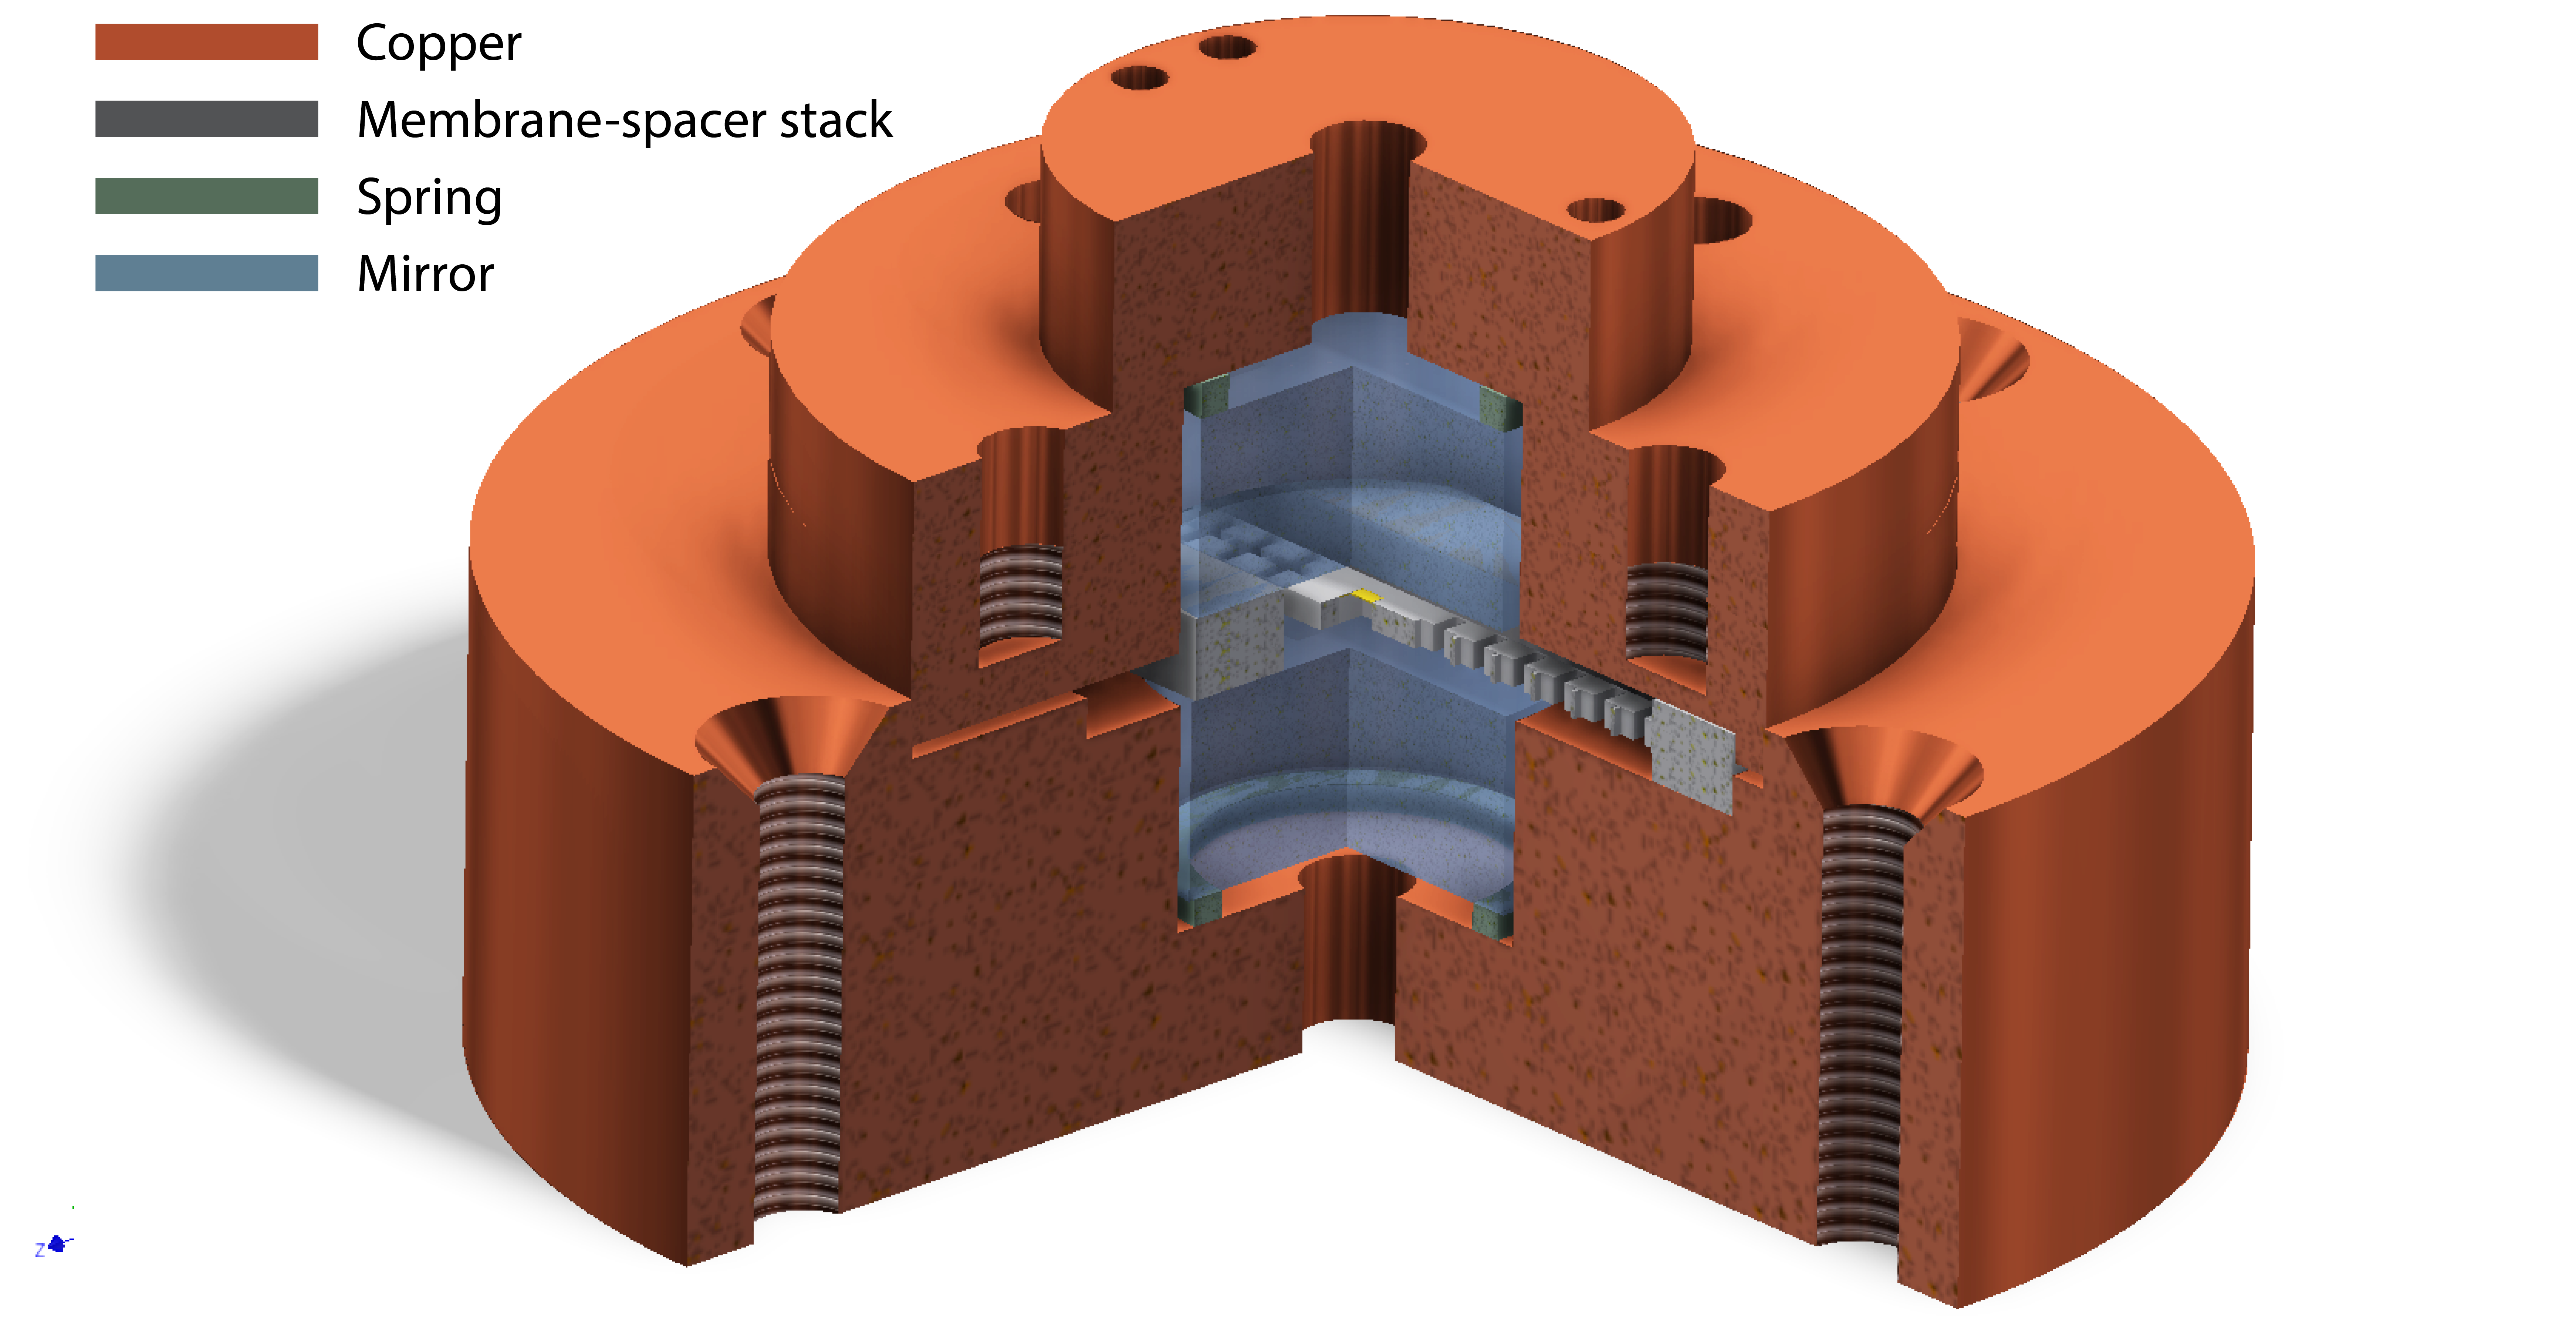
\includegraphics[scale=0.2]{bigBud_v09_new.png}
\caption{Fully assembled sample holder.}
\label{fig:sample_holder_tilt}
\end{figure}

Let us describe the sample holder's three parts piece by piece, starting with the bottom part. It is \SI{30}{\milli\meter} in diameter and has four threaded holes, matching holes in the cold finger, such that it can be firmly anchored in the cold finger of the cryostat and act as good thermal bridge to the rest of the sample holder. A small hole going all the way through with \SI{2}{\milli\meter} in diameter is placed in the middle, allowing for light to pass through, but with a small enough angle of incident, so as to limit thermal radiation. The hole for the spring and flat bottom mirror are machined to have the quarter inch mirror sticking a bit out of the hole (dependent on choice of spring), such that the membrane stack can compress the spring and enable parallelism between mirror and membrane surface. A small groove to fit the membrane stack is made to account for alignment of the membrane, but since the couple first generation of membranes chips did not have well defined edge dimensions, the size of the groove's length dimensions was extended to accommodate for this uncertainty and in the end made alignment more difficult. Four threaded holes for the middle part to fasten and a little groove for the middle part to fit in is cut. The middle part can be hard to separate from the top part in figure \ref{fig:sample_holder_tilt}, for more details see figure \ref{fig:sample_holder_pull}, where the sample holder parts are pulled apart. The middle part is a disk \SI{20}{\milli\meter} in diameter. On the side facing towards the bottom part there is also a small grove like the one in the bottom part to align the membrane stack. The middle part pushes the membrane stack and compresses the bottom spring when screwed into the bottom part. The membrane stack then gets thermalized through the middle piece. A hole is machined in the middle where the top curved mirror is placed. The four tiny holes in pairs of two is to allow air to escape upon evacuation of the cryostat. The top part can be fastened to the middle part. It looks like a hat and it is in fact hollow, such that it can glide down on the top mirror with a spring placed on top. There is a small \SI{2}{\milli\meter} hole for incoupling in the top part as well.

\begin{figure}[H]
\centering
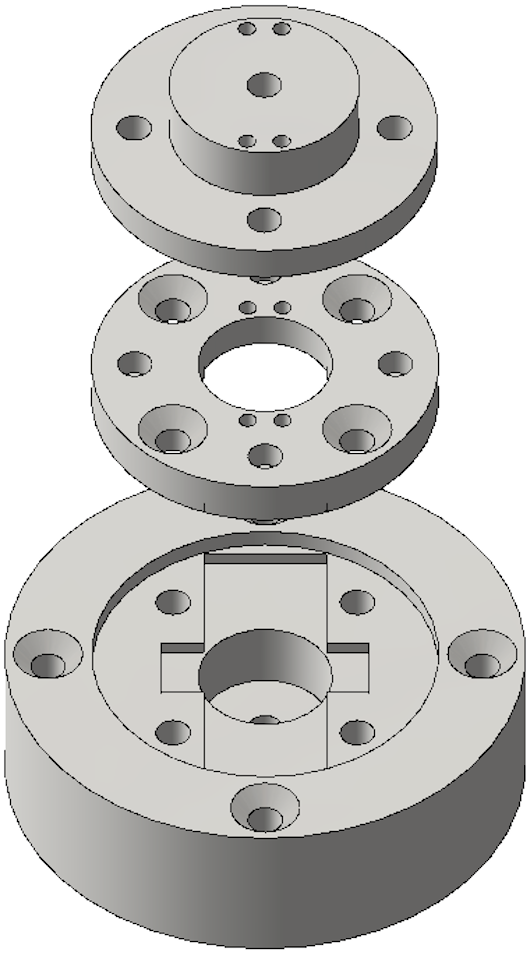
\includegraphics[scale=0.5]{side_topv2.png}
\caption{Sample holder pulled apart. The color scheme is changed to grey scale for better detail outline.}
\label{fig:sample_holder_pull}
\end{figure}

The sample chips have a height of \SI{0.5}{\milli\meter}, and thus the spacer-membrane-spacer stack is roughly the cavity length of $L \approx 1.5$ \SI{}{\milli\meter}. As springs we use thin copper washers custom bent in three places to form a wave spring. See figure \ref{fig:sample_holder_inside} for assembly inside the sample holder.

\begin{figure}[H]
\centering
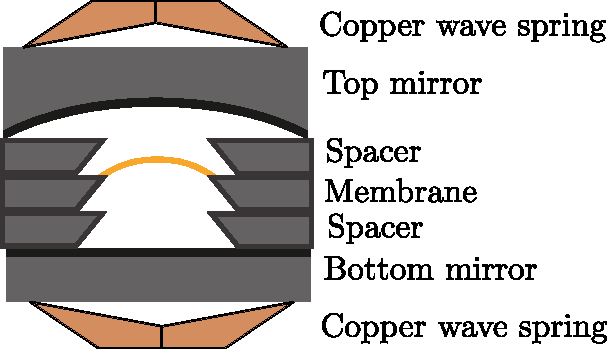
\includegraphics[scale=0.7]{mim_setup.pdf}
\caption{Assembly inside the sample holder.}
\label{fig:sample_holder_inside}
\end{figure}

A thing that we did not anticipate, was that we would need to push around the top mirror horizontally to finally align the cavity. The hope was that the geometry of the sample holder solved this problem, but sadly it did not. To enable this degree of freedom, we drilled four small opposite holes in sides of the top part of the sample holder, allowing for small metal rods to push the top mirror around. We called it the ``pinhead" solution. It was somewhat cumbersome, but it got the job done.

By a communication error we ended up having the sample holder made in the material Elmedur, which is another alloy of copper instead of oxygen-free copper. This mistake was first realized after the data was taken.